\documentclass[10pt,a4paper]{amsart}
\usepackage[margin=19mm]{geometry}
\usepackage{amsmath,amssymb,mathtools}
\usepackage[scr=rsfs,cal=euler]{mathalfa}
\usepackage{xfrac}
\usepackage[unicode,hidelinks,bookmarks=false]{hyperref}
\newcommand{\ie}{i.e.\ }
\newcommand{\cf}{cf.\ }
\newcommand{\resp}{respectively\ }
\newcommand{\Subsection}{\subsection}
\providecommand{\nobreakdash}{\nobreak\hbox{-}}
\setlength{\emergencystretch}{2em}
\multlinegap0pt
\usepackage{tikz}
\usepackage{amssymb}
\usepackage{subfig}
\usepackage[all]{xy}
\usepackage{csquotes}
\newtheorem{lemma}{Lemma}
\title{On balance properties of hypercubic billiard words}
\author{Nicolas B\'edaride, Val\'erie Berth\'e, Antoine Julien}
\date{Source: arXiv:2502.18211v2 (CC BY 4.0)}
\begin{document}
\maketitle

\noindent\emph{Source and licence.} On balance properties of hypercubic billiard words. Version arXiv:2502.18211v2 (CC BY 4.0), distributed by arXiv under the Creative Commons Attribution 4.0 International licence, http://creativecommons.org/licenses/by/4.0/, as recorded in the arXiv licence metadata for this exact version and shown on the abstract page https://arxiv.org/abs/2502.18211v2. Full licence notice: \texttt{licenses/arxiv-2502.18211-CC-BY-4.0.txt}.\par\smallskip

\noindent\textit{Editorial scope.} Counted unit: the article's lemma lemma (source0.tex lines 1527--1529). The article's complete original proof of it is delivered with it (source0.tex lines 1530--1577, one \texttt{proof} environment of 48 lines). No mathematics is written, repaired or re-derived: the statement and the proof are the article's own lines, in the article's own notation, and no retained line is substituted or re-flowed.  No further source-local context is needed: every cross-reference of every retained line resolves inside the two delivered spans.  Nothing was omitted from any retained span, so the package carries no omission record.  No retained line contains a citation, so the wrapper carries no bibliography and no bibliography entry.  The retained lines contain the article's own diagram code, which the wrapper typesets with the standard tikz packages; no image file is delivered and the package declares no asset dependency.  Editorial formatting only, in addition: an AMS \texttt{amsart} preamble that restates the article's own declarations and macros used by the retained lines, namely the environments \texttt{lemma} on separate counters, together with the standard packages those lines need.  The retained environments print in this document as Lemma 1 in order of appearance, whereas the article prints the same items with the numbering of its own full document.  The complete native source of the article as distributed in the arXiv e-print for this exact version is bundled unchanged as \texttt{sources/173836/source0.tex}.
\begin{lemma}
The volume of each of these polyhedra doe not belong to $\mathbb Q(\theta_1,\dots, \theta_4)$.
\end{lemma}

\begin{proof}

On prend la direction $\theta=\begin{pmatrix}1\\u_1\\ u_2\\u_3\end{pmatrix}$ et on regarde la matrice de projection sur $\theta^\perp$. 
On trouve
$$\frac{1}{1+u_1^2+u_2^2+u_3^2}\begin{pmatrix} u_1^2+u_2^2+u_3^2&-u_1&-u_2&-u3\\
-u_1&1+u_2^2+u_3^2&-u_2u_1&-u_1u_3\\
-u_2&-u_1u_2&1+u_1^2+u_3^2&-u_2u_3\\
-u_3&-u_1u_3&-u_2u_3&1+u_1^2+u_2^2
\end{pmatrix}$$

Les $4$ colonnes sont les 4 vecteurs $f_1,\dots,f_4$ qui vérifient bien $$f_1+u_1f_2+u_2f_3+u_3f_4=0.$$ Ces vecteurs se retrouvent dans la figure comme suit
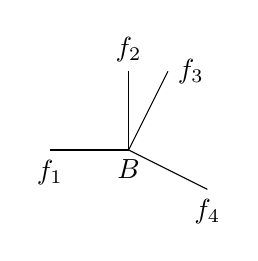
\begin{tikzpicture}
\draw (-1,0)--(0,0)--(0,1);
\draw (1,-1/2)--(0,0)--(1/2,1);
\draw (0,0) node[below]{$B$};
\draw (-1,0) node[below]{$f_1$};
\draw (0,1) node[above]{$f_2$};
\draw (1/2,1) node[right]{$f_3$};
\draw (1,-1/2) node[below]{$f_4$};
\end{tikzpicture}
Le cube engendré par $F_i, f_j, f_k$ avec $i\neq j\neq k$, a pour volume 
$$|f_i||^2||f_j||^2||f_k||^2-<f_i,f_j>^2||f_k||^2-<f_i,f_k>||f_j||^2$$

 
Pour avoir le volume des petits polyèdres il faut trouver les coordonnées des points $C$, {\it etc}. 
Cela revient à avoir
$$A=f_1+f_2+f_4+f_3, B=0$$

$C=f_4+f_3+f_2+f_1-\lambda f_3=af_1+bf_2$. 
$$C=f_4+(1-\lambda) f_3+(1-a)f_1+(1-b)f_2=0=f_1+u_1f_2+u_2f_3+u_3f_4=0$$
La relation de dependance permet de conclure aux coordonnées de $C$.
$$\lambda=u_2/u_3-1, a=1/u_3-1, b=u_1/u_3-1.$$

On considère le polytope ayant pour sommets $A, B, C$. C'est un parallélépipède, donc son volume vaut 
$$ab\lambda Vol(f_1,f_2,f_3)$$ 
$$\frac{(1-u_3)(u_2-u_3)(u_1-u_3)}{u_3^3}Vol(f_1,f_2,f_3)$$ 

$$\frac{(1-u_3)(u_2-u_3)(u_1-u_3)}{u_3^2}$$ 
 \maltese\maltese On raisonne par l'absurde: Il faudrait que ce nombre soit combinaison linéaire de $1,u_1,u_2, u_3$.
 ?????
 
 \maltese\maltese
 

Calcul des autres volumes: assez complexe...Décomposer en pyramides. Seuls polyèdres dont je connais le volume:
Pyramide: $1/3*B*h$ et parallélépipède: $B*h$.

\end{proof} 

\end{document}
